\documentclass[border=4mm]{standalone}
\usepackage{pgfplots}
\usepackage{helvet}
\renewcommand{\familydefault}{\sfdefault}
\pgfplotsset{compat=1.18}
\begin{document}
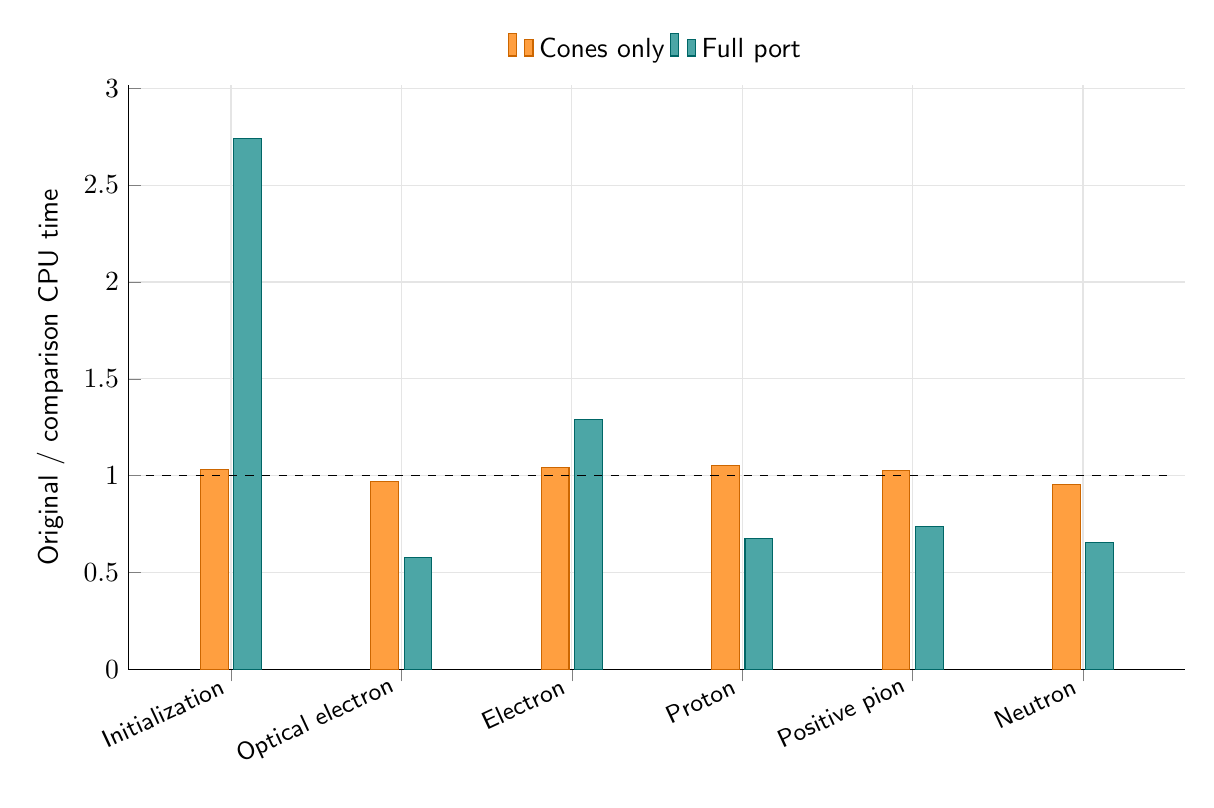
\begin{tikzpicture}
\begin{axis}[width=15cm,height=9cm,ybar,bar width=10pt,
 ylabel={Original / comparison CPU time},ymin=0,
 xtick={0,1,2,3,4,5},xticklabels={Initialization,Optical electron,Electron,Proton,Positive pion,Neutron},
 x tick label style={rotate=25,anchor=east,font=\small},
 grid=major,major grid style={gray!20},axis lines*=left,
 legend style={at={(0.5,1.02)},anchor=south,legend columns=2,draw=none},
 enlarge x limits=0.12]
\addplot[fill=orange!75,draw=orange!80!black] coordinates {
(0,1.032418) (1,0.970759) (2,1.042366) (3,1.054112) (4,1.026823) (5,0.956494)
};
\addplot[fill=teal!70,draw=teal!80!black] coordinates {
(0,2.740238) (1,0.577652) (2,1.288043) (3,0.677638) (4,0.738916) (5,0.655664)
};
\addplot[black,dashed,sharp plot,update limits=false] coordinates {(-0.5,1) (5.5,1)};
\legend{Cones only,Full port}
\end{axis}
\end{tikzpicture}
\end{document}
